\chapter{项目展示}

\section{教程版块}

用户可以查看公开的以及分享给自己的教程,教程的可读权限和可写权限是在创建教程时给定的,教程支持Markdown和Latex渲染,内嵌了程序的可执行环境。教程详情页面如下:

\begin{figure}[H]
    \centering
    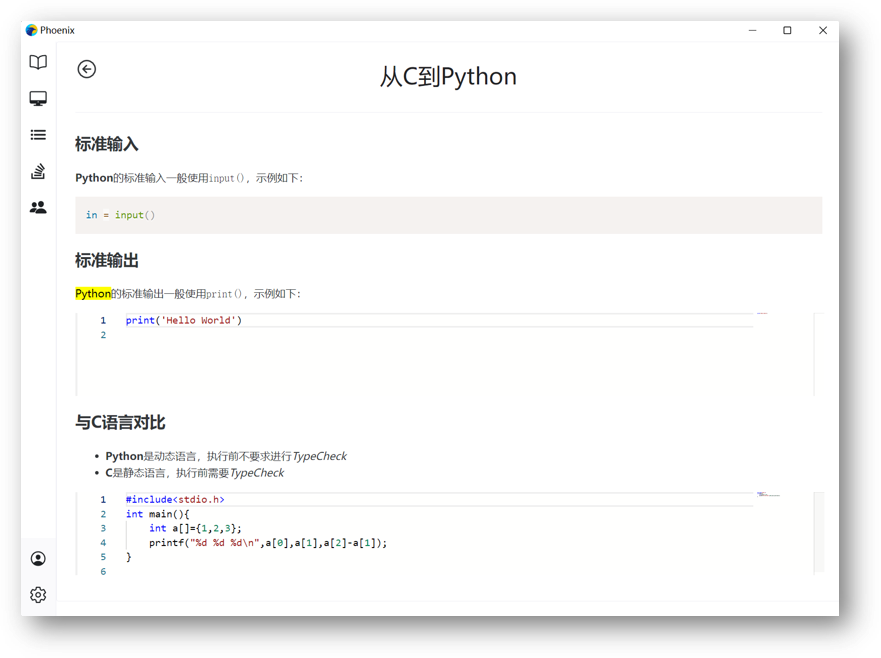
\includegraphics[width=0.7\textwidth]{figure/tutorial1.png}
    \caption{\textbf{教程详情页面}}
    \label{fig:tutorial1}
\end{figure}

\section{比赛版块}

组织管理员可以通过选择题目创建比赛,比赛可以指定允许参加比赛的用户范围、比赛开启的时间等内容。创建比赛页面如下:

\begin{figure}[H]
    \centering
    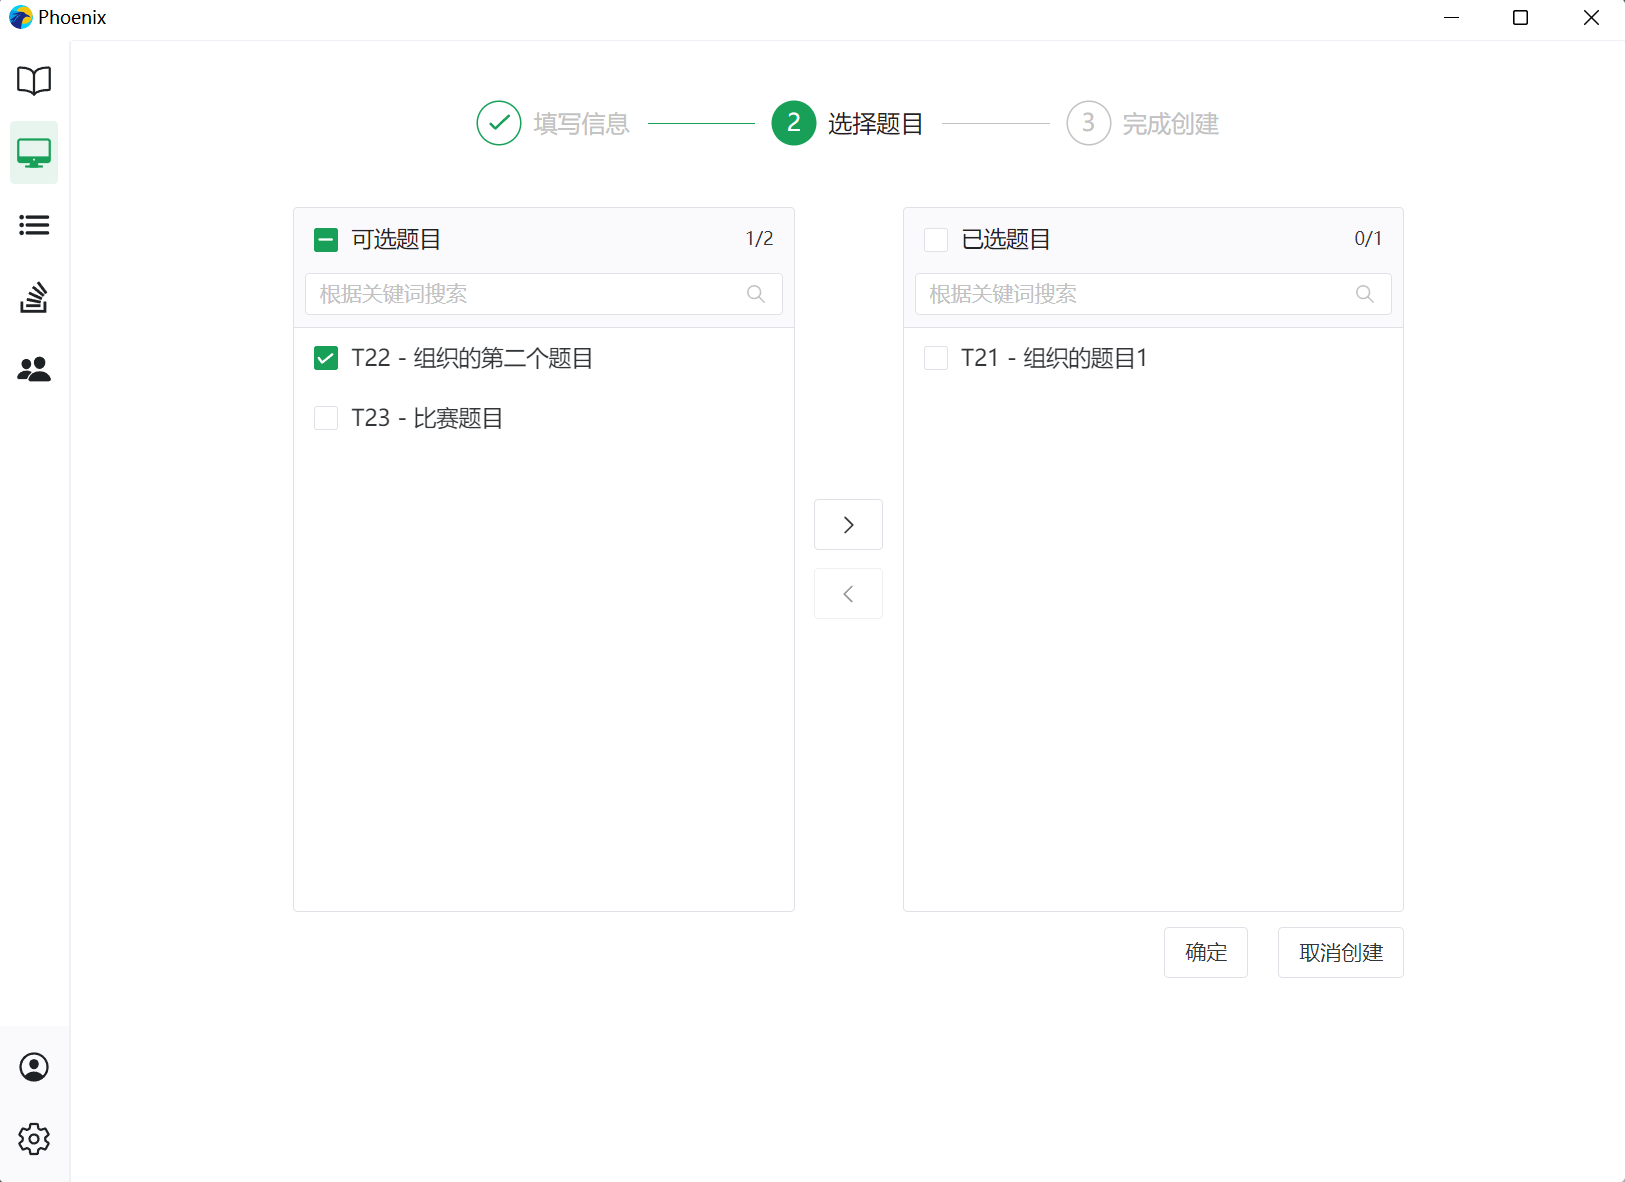
\includegraphics[width=0.7\textwidth]{figure/contest1.png}
    \caption{\textbf{创建比赛页面}}
    \label{fig:contest1}
\end{figure}

在允许参赛范围内的用户可以参加比赛,比赛过程中系统可以实时排名,比赛详情页面如下:

\begin{figure}[H]
    \centering
    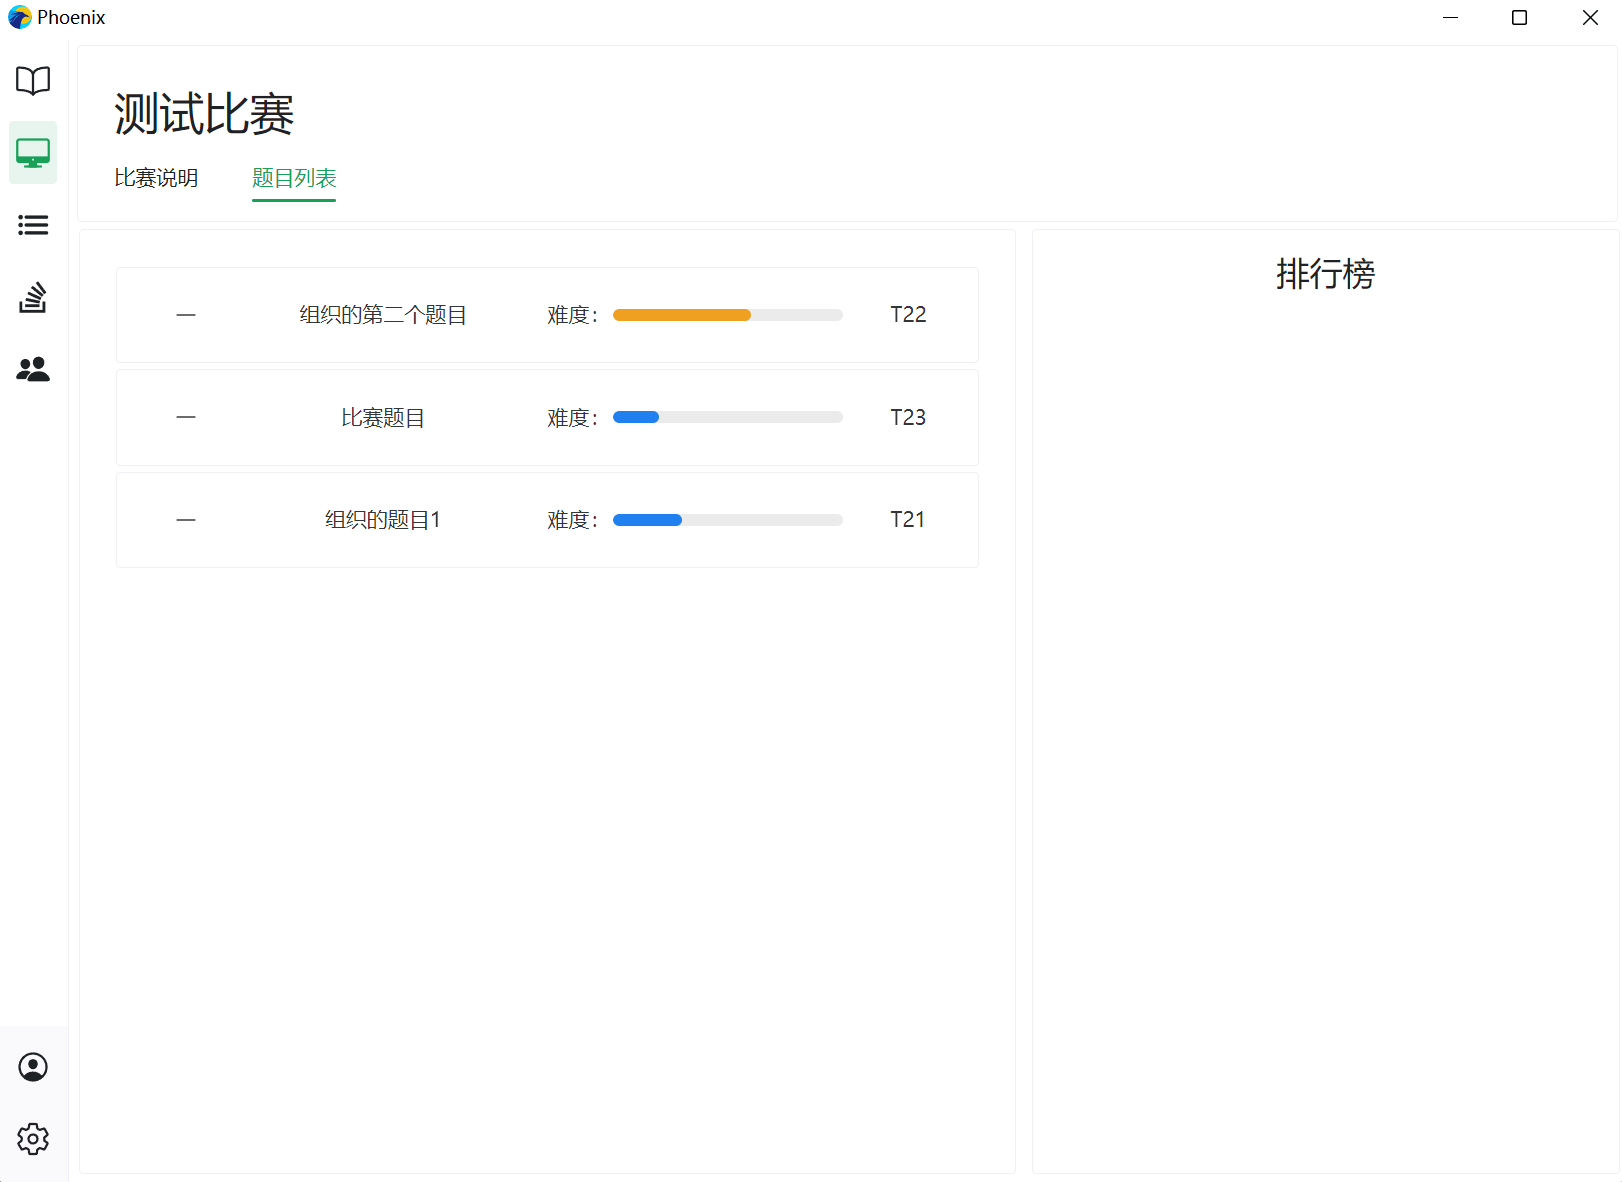
\includegraphics[width=0.7\textwidth]{figure/contest2.png}
    \caption{\textbf{比赛详情页面}}
    \label{fig:contest2}
\end{figure}

\section{评测版块}

用户可以查看具有读权限的所有题目,题目列表中会标明题目的难度、名称、通过情况等信息,题目列表页面如下:

\begin{figure}[H]
    \centering
    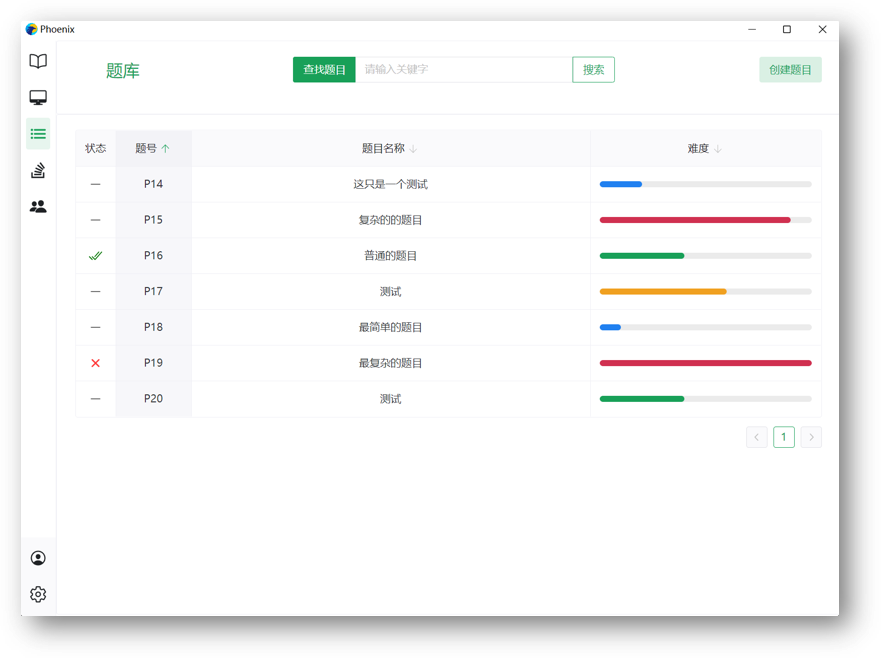
\includegraphics[width=0.7\textwidth]{figure/problem1.png}
    \caption{\textbf{题目列表页面}}
    \label{fig:problem1}
\end{figure}

用户可以查看自己的历史评测记录,并下载自己的评测文件,评测记录页面如下:

\begin{figure}[H]
    \centering
    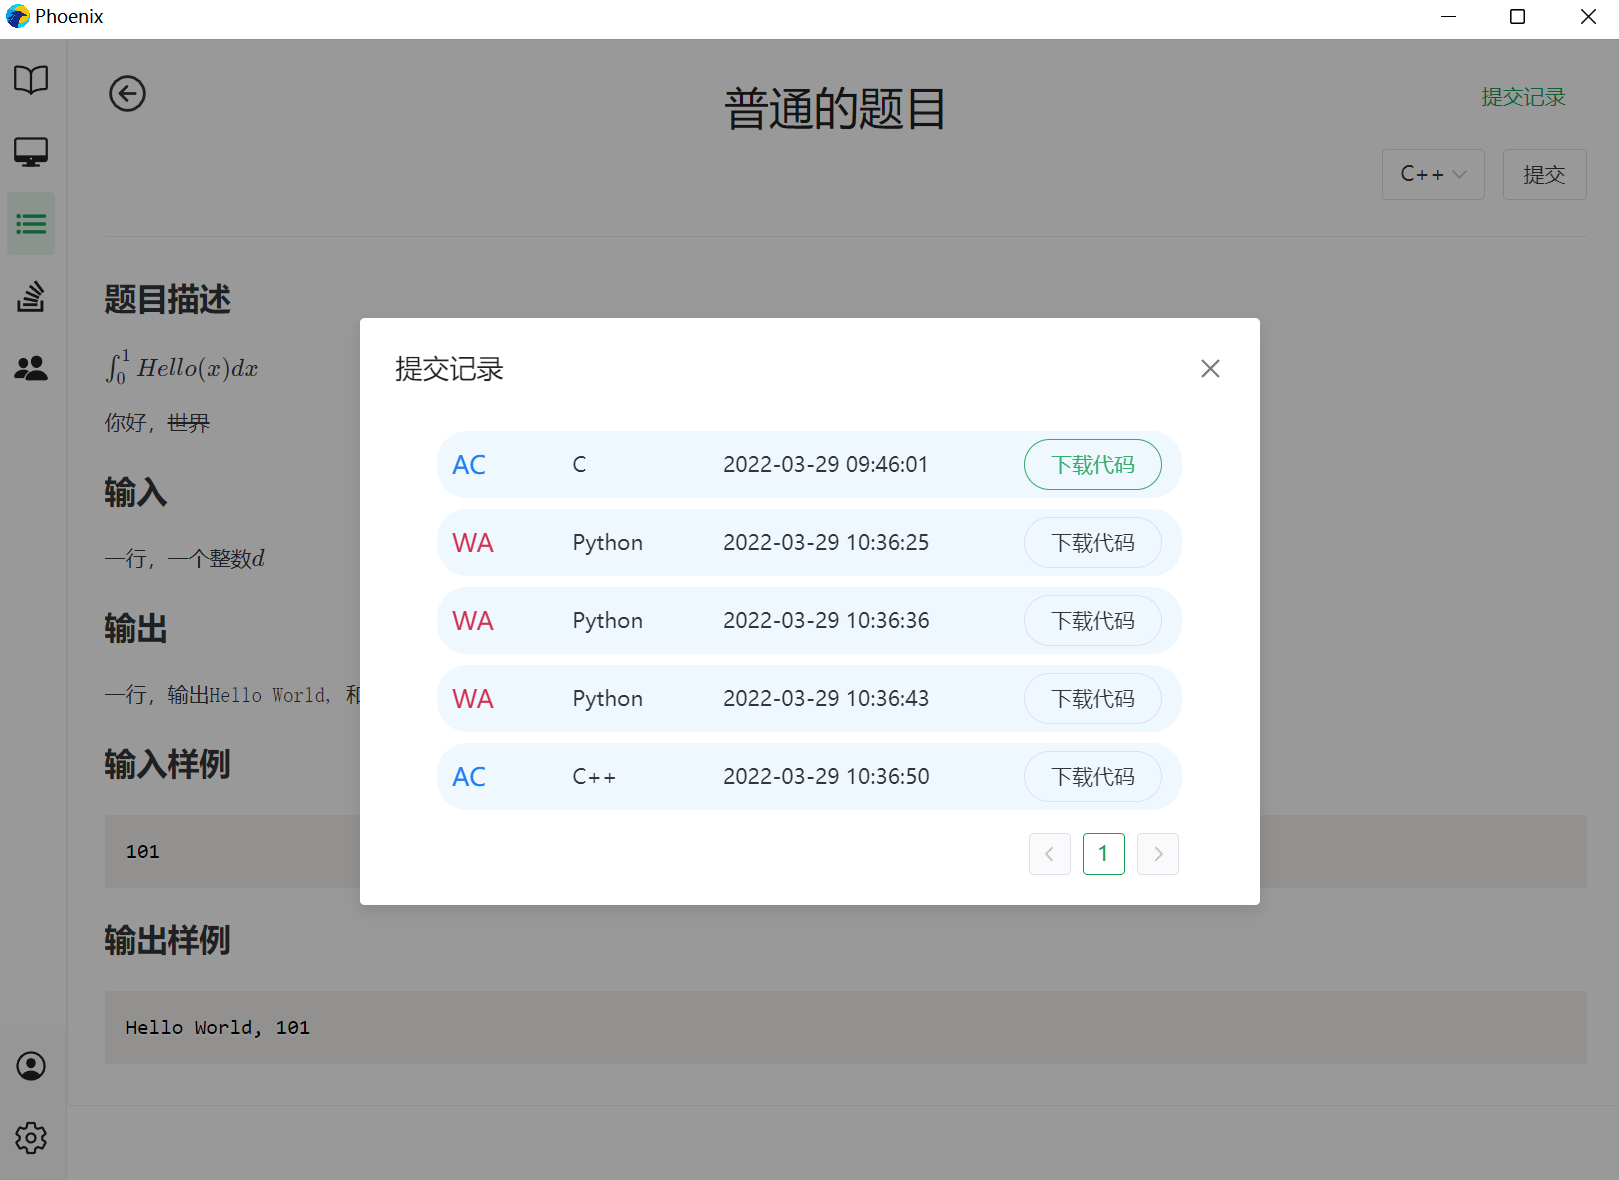
\includegraphics[width=0.7\textwidth]{figure/problem2.png}
    \caption{\textbf{评测记录页面}}
    \label{fig:problem2}
\end{figure}

\section{论坛版块}

每个组织都有自己的论坛,用户可以在论坛内交流。论坛内置不同的版块,用于放置不同的讨论内容,论坛页面如下:

\begin{figure}[H]
    \centering
    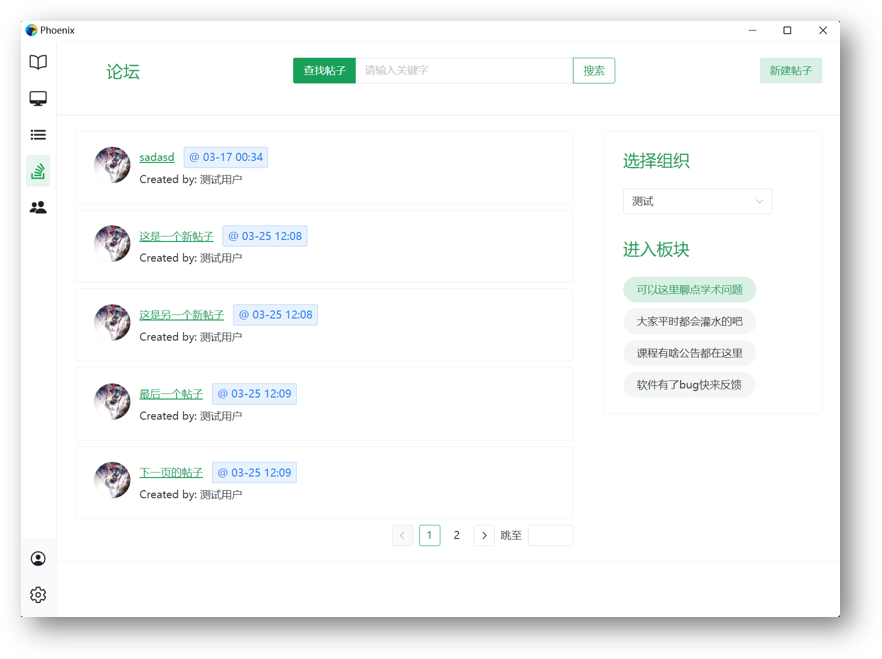
\includegraphics[width=0.7\textwidth]{figure/forum1.png}
    \caption{\textbf{论坛页面}}
    \label{fig:forum1}
\end{figure}

\section{组织管理版块}

用户可以查看自己所属的所有组织,实时查看自己收到的组织邀请,组织列表页面如下:

\begin{figure}[H]
    \centering
    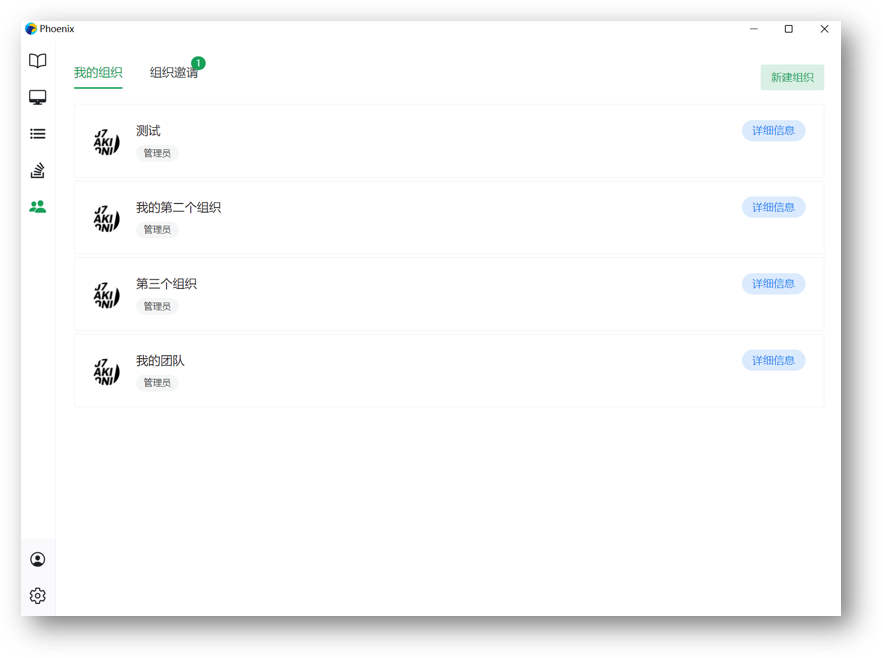
\includegraphics[width=0.7\textwidth]{figure/team1.png}
    \caption{\textbf{组织列表页面}}
    \label{fig:team1}
\end{figure}

组织管理员可以管理自己的组织,可以设置组织成员的权限,设置组织的相关信息,组织管理页面如下:

\begin{figure}[H]
    \centering
    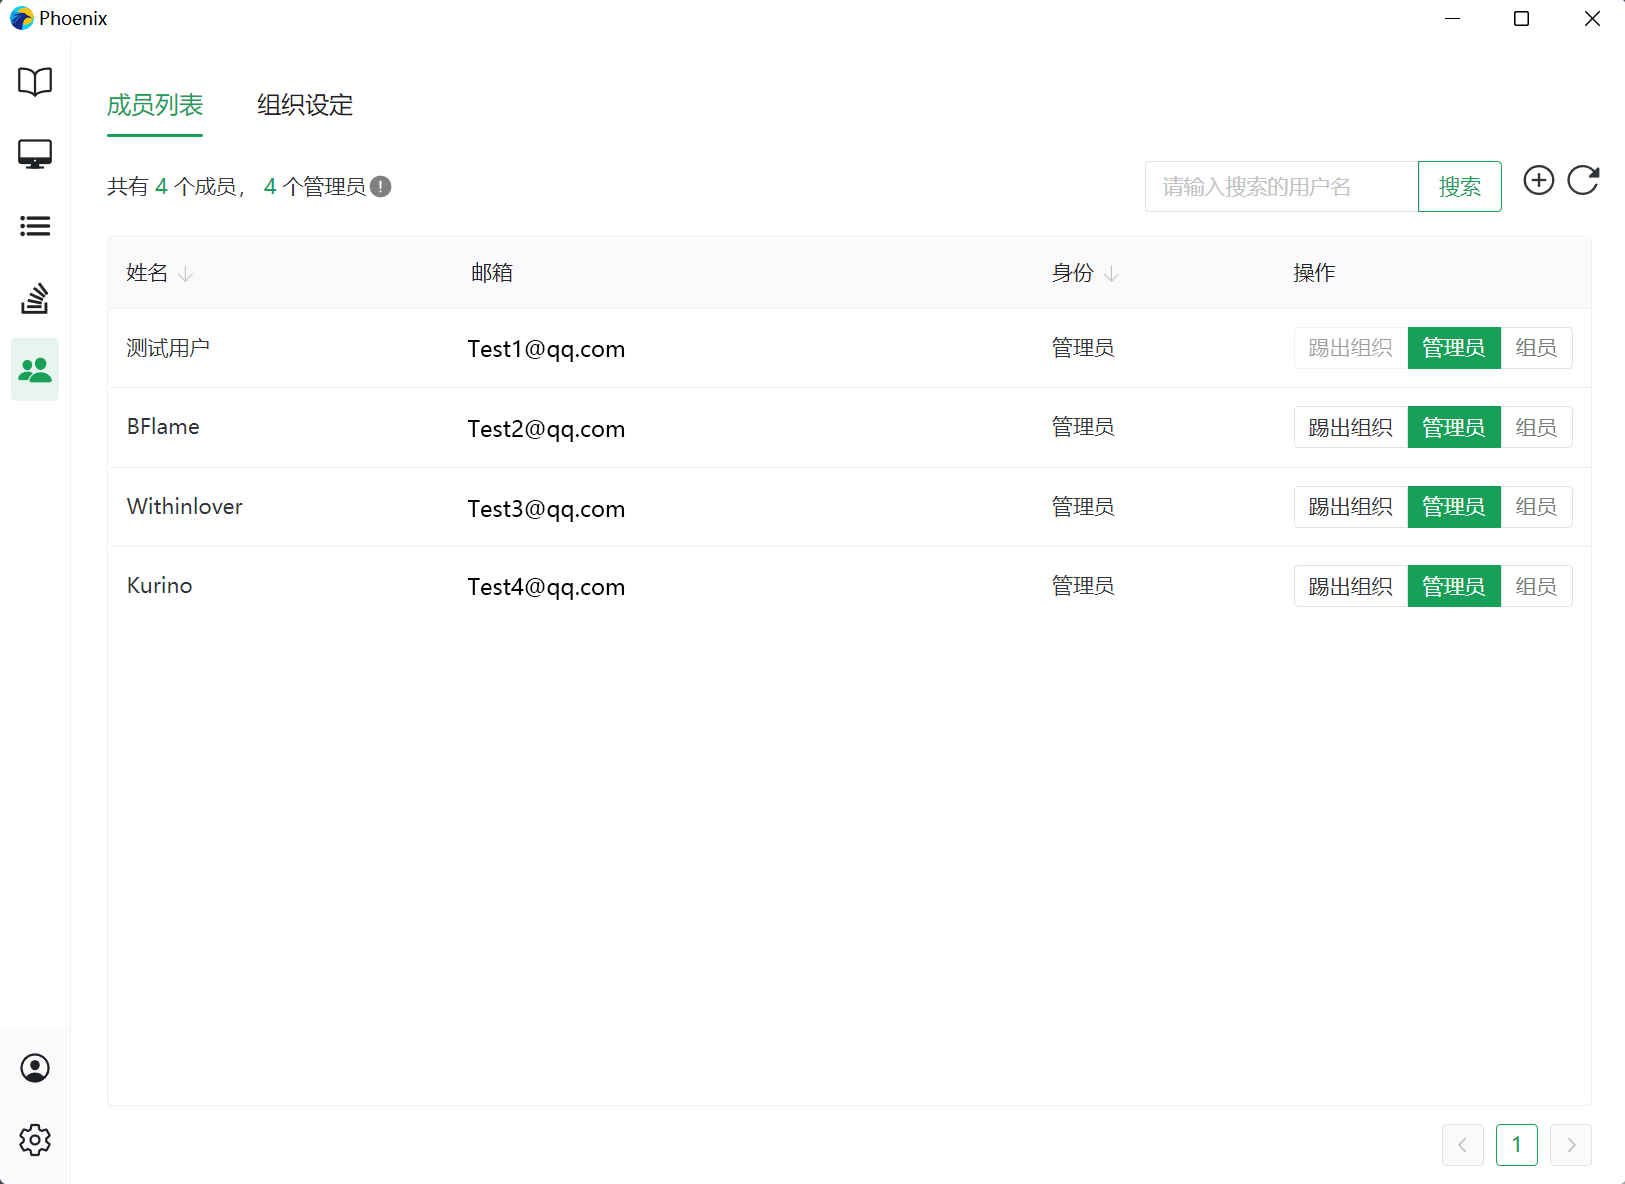
\includegraphics[width=0.7\textwidth]{figure/team2.png}
    \caption{\textbf{组织管理页面}}
    \label{fig:team2}
\end{figure}
